\documentclass[12pt]{article}
\usepackage[utf8]{inputenc}
\usepackage[T2A]{fontenc}
\usepackage[russian]{babel}
\usepackage{amsmath}
\usepackage{amsfonts}
\usepackage{mathtools}
\usepackage{graphicx}
\usepackage{color}
\usepackage{MnSymbol}
\usepackage{array}
\usepackage{stackengine}
\usepackage[a4paper, total={6in, 8in}]{geometry}
\title{Математический анализ 2-ой семестр}
\author{Никитская Варвара}
\ignorespacesafterend 
% Start the document
\begin{document}
\tableofcontents
\newpage
% Create a new 1st level heading
\section{Векторные пространства}
\subsection{Основные понятия и утверждения}

\textbf{Опр.} Множество V называется векторным пространством над полем F, если на V введены операции: + $\forall (v_1, v_2) \in VxV \rightarrow v \in V$ и $\lambda \bullet$ $\forall (\lambda, b) \rightarrow \lambda v \in V$, удовлетворяющие следующим аксиоам:
\begin{enumerate} 
\item $v_1, v_2, v_3 \in V: v_1+(v_2 + v_3) = (v_1 + v_2) + v_3$ 
\item $\exists 0 \in V: \forall v \in V: v + 0 = 0 + v = v$
\item $\forall v \in V: \exists -v \in V: v + (-v) = -v + v = 0$
\item $\forall v_1, v_2 \in V: v_1 + v_2 = v_2 + v_1 $
\item $\lambda_1(\lambda_2 v) = (\lambda_1\lambda_2 )v$
\item 1v=v1=v
\item $\lambda (v_1 + v_2) = \lambda v_1 + \lambda v_2$
\item $(\lambda_1 + \lambda_2 )v = \lambda_1 v + \lambda_2 v$
\end{enumerate}

\textbf{Опр.} $v \in V$ - вектор
\newline

\textbf{Опр.} $\lambda \in F$ - скаляр
\newline

\textbf{Опр.} Пусть $U \subset V$ - векторной подпространства пространства V, если U само является векторным пространством относительно операций, заданных в V.
\newline 

\textbf{Утв.} Это определение равносильно: 
\begin{enumerate}
\item $U \ne \emptyset$ 
\item $v_1 + v_2 \in U, \forall (v_1,v_2) \in U$
\item $\forall \lambda \in F, \forall v \in U: \lambda v \in U$
\end{enumerate}

\textbf{Опр.} Векторы $v_1\cdots v_n \in V$ называются линейнозависимыми, если $\exists \lambda_1\cdots\lambda_n\in F$ (не все нули): $\lambda_1 v_1 + \cdots + \lambda_n v_n = 0$
\newline

\textbf{Утв.} Это определение равносильно тому, что один из векторов линейно выражается через остальные.
\newline

\textbf{Опр.} Упорядочеенный набор $v_1,v_2\cdots v_n \in V: e$ называется базисом в V, если это максимальный линейнонезависимый набор.
\newline

\textbf{Утв.} e является базисом в V $\Leftrightarrow e_1\cdots e_n$ - ЛНЗ и $\forall v\in V \exists\lambda_1\cdots\lambda_n\in F: v = v_1\lambda_1 + \cdots + v_n\lambda_n$ 
\newline

\textbf{Обозначим} $X_e = \begin{pmatrix} x_1 \\ \vdots \\ x_n \end{pmatrix} \in F$ тогда $x =eX_e$.
\newline

\textbf{Теорема:} если в V существует базисиз n векторов, то во всех базисах V содержится n векторов.\newline
\textbf{Доказательство:} через основную лемму о линейной зависимости (см. 1 семестр)
\newline

\textbf{Опр.} пусть dimV=n, e-исходный базис, e'-новый базис $\Rightarrow$ $\forall j=1\cdots n: \newline e_j'=\displaystyle\sum_{i=1}^n e_{ij}e_j$. С - матрица перехода, где по столбцам написаны координаты векторов нового базиса в старом. $e'=(e_1\cdots e_n)C_{e\to e'}$
\newline

\textbf{Свойства матриц перехода:}
\begin{enumerate}
\item C - невырожденная 
\newline \textbf{Доказательство:} Столбцами C являются столбцы ЛНЗ векторов $e_1'\cdots e_n' \Rightarrow detC \ne 0$
\item $C_{e'\to e} = C^-1_{e\to e'}$
\newline \textbf{Доказательство:} По определению матрицы перехода $e' = (e_1'\cdots e_n') = (e_1\cdots e_n)C_{e\to e'}$ С другой стороны $e = (e_1'\cdots e_n')C_{e'\to e}$. Ввиду единственности разложения по базис $C_{e\to e'}C_{e\to e} = E$
\item $C_{e\to e''} = C_{e\to e'}C_{e'\to e''}$
\newline \textbf{Доказательство:} По определению $e''=e'C_{e'\to e''}=eC_{e\to e'}C_{e'\to e''} = eC_{e\to e''} \Rightarrow C_{e\to e''} = C_{e\to e'}C_{e'\to e''}$

\end{enumerate}

Как выглядит матрица перехода, если известны координаты $e_i$ и $e'_j$ в универсальном базисе E. Можно рассмотреть матричное уравнение: $(e_1^{\uparrow}\cdots e_n^{\uparrow})C = (e_1^{'\uparrow}\cdots e_n^{'\uparrow}). \newline [e_1^{\uparrow}\cdots e_n^{\uparrow} | e_1^{'\uparrow}\cdots e_n^{'\uparrow}] \stackrel{\text{ЭП}}{\leadsto} \left[E|C\right]$
\newline

Изменение координат вектора при замене базиса: $X_e = C_{e\to e'}X_{e'}$
\newline \textbf{Доказательство:} $\forall x\in V, x=eX_e=e'X_{e'}=eC_{e\to e'}X_{e'}$, ввиду единственности разложения по базиу e, $X_e=C_{e\to e'}X_{e'}$ 

\subsection{Подпространства}

\textbf{Типовые примеры:}
\newline

0. Геометрические векторы
\begin{enumerate} 
\item $F^n$ пространство столбцов (или  строк) высоты (длины) n, с естественным операциями. Базис - $\begin{pmatrix} 1\\ \vdots \\ 0\end{pmatrix} \cdots \begin{pmatrix} 0\\ \vdots \\ 1\end{pmatrix}$
\item $M_{mxn}(F)$ с естественным операциями. $dim M_{mxn} = mn$. Стандартный базис из всех матричных единиц.
\item $V=\{f: x\to \mathbb{R}\}$ с операциями поточечность сложения и умножения на скаляр. V бесконечномерное, если x бесконечно.
\item $F[t]$ с  естественными операциями. Бесконечномерное $\forall n \in \mathbb{N}_0: 1,t,\cdots ,t^n$ - ЛНЗ. $F[t]_n = \{a_0+a_1t+\cdots+a_nt^n\} a_i\in F i=\{1\cdots n\}$ - подпространство размерности n+1. Базис: $1,t,\cdots ,t^n$. Тейлорский базис: $1, t-t_0,\cdots ,(t-t_0)^n$
\item $\Omega \ne 0. V=2^{\Omega}$ с операцией вместо сложения $A\Delta B = (A\cap \overline{B}) \cup (B \cap \overline{A}) \forall A,B \in \Omega$, $F=\mathbb{Z}_2: 0A=\emptyset , 1A = A$ 
\end{enumerate}

Два основных способа задания подпространства в V:
\begin{enumerate}
\item Линейная оболочка семейства векторов $S\subset V$. $<S>=\{\sum_{i\in I}\lambda_i S_i\} (\text{конечная сумма}), s_i\in S, \lambda_i\in F.$ \newline

Частный случай: $<a_1\cdots a_n>=\{\sum_{i\in I}\lambda_i a_i\} \lambda_i \in F$. \newline

\textbf{Утв.} $<a_1\cdots a_n> \subset V, dim<a_1\cdots a_n> = rk\{a_1\cdots a_n\}$
\newline \textbf{Доказательство:} \begin{enumerate} 
\item $\mu\sum_{i=1}^m\lambda_i a_i + \sum_{i=1}^m\mu\lambda_i a_i$
\item $\sum_{i=1}^m\lambda_i a_i + \sum_{i=1}^n\mu_i a_i =\sum_{i=1}^k (\lambda_i + \mu_i )a_i$ $\Rightarrow$ набор векторов a - подпространство в V. 
\end{enumerate}
Если $r=rk\{a_1\cdots a_n\}$ и $a_k\cdots a_s$ - базисные, то любой вектор $a_i$ выражается через них $\Rightarrow$ любая линейная комбинация тоже $\Rightarrow a_k\cdots a_s$ базис. (конец док. утв.)

Алгоритм вычисления $dim<a_1\cdots a_n>$ и базиса, если известны координаты этих векторов: составляем матрицу $(a_1^{\uparrow}\cdots a_n^{\uparrow})$, приводим к улучшенному ступеньчатому виду с помощью ЭП над строками, тогда столбцы с лидерами - базисные вектора. Разложение остальных находятся с помощью коэффициентов свободных членов.

\item dimV = n известны координаты в некотором базис $\forall x=\sum_{i=1}^n x_i e_i = eX$
W = $\{x=eX | AX = 0\}$ - решения ОСЛУ. \newline
\textbf{Утв.} W - подпространство в W. dimW = n-rkA. Базис - любая ФСР. 
\end{enumerate}

\textbf{Теорема} Линейную оболочку конечного числа векторов в конечномером векторном пространстве V можно задать с помощью ОСЛУ.
\newline \textbf{Доказательство:} два способа: 
\begin{enumerate}
\item Вектор х со столбцом координат $X=\begin{pmatrix} x_1 \\ \vdots \\ x_n \end{pmatrix}$. \newline $x \in <a_1\cdots a_m> \Leftrightarrow \exists \alpha_i\cdots\alpha_m\in F: \sum_{i=1}^m\alpha_i a_i=x$ или в координатах: $\sum_{i=1}^m\alpha_i a_i^{\uparrow}=X$ то есть СЛУ с $\overline{A} = \left(a_1^{\uparrow}\cdots a_m^{\uparrow} | \begin{matrix} x_1 \\ \vdots \\ x_m \end{matrix} \right)$ совместна $\Leftrightarrow$ после алгоритма Гаусса $\overline{A} \stackrel{\text{усв}}{\leadsto} \begin{pmatrix} 1 & * & \cdots & * & | & \sum C_{rj}x_{j} \\ 0 & 1 & \cdots & * & | &  \\ 0 & 0 & 1 & * & | &  \\ \hline \\ 0 & 0 & 0 & 0 & | & \sum C_{r+1,j}x_j \\ 0 & 0 & 0 & 0 & | & \sum C_{n,j}x_j \end{pmatrix}$ (сумма при нулевых строках - нужная нам ОСЛУ, где r - ранг матрицы).
\item Пусть дана ОСЛУ CX = 0 (где у С r строк). $C \stackrel{\text{*}}{\leadsto} \begin{pmatrix} 1 & \cdots & 0 & | &  \\ 0 & \cdots & 0 & | & \\ \vdots & \vdots & \vdots & | &  D \\ 0 & \cdots & 0 & | & \\ 0 & \cdots & 1 & | & \\ \end{pmatrix}$ = C' = $(E_r | D)$
$$\begin{cases} x_1 = d_{1r+1}x_{r+1} + \cdots + d_{1n}x_n \\ \cdots \\ x_k = d_{kr+1}x_{r+1} + \cdots + d_{kn}x_n \end{cases} (k=1\cdots r)$$

Фундаментальная матрица $T = \begin{pmatrix} -D \\ \hline \\ E_{n-r}\end{pmatrix}$ $C'T = E_r(-D) + DE_{n-r} = -D + D = 0 \Rightarrow$ Фундаментальная матрица - это решения исходной ослу. \newline 
Мы доказали, что фундаментальная матрица является решением подобной ослу. Теперь рассмотрим нужную нам фундаментальную матрицу из базисных векторов $a_1\cdots a_r$, запишем их по строчкам:\newline 
$\begin{pmatrix} a_1^{\rightarrow} \\ \vdots \\ a_r^{\rightarrow} \end{pmatrix} \stackrel{\text{*}}{\leadsto}\begin{pmatrix} M_{rx(n-r)} & \vline & E_r \end{pmatrix} \stackrel{\text{транспонирование}}{\rightarrow}\begin{pmatrix}M^T \\ \hline \\ E_r \end{pmatrix} = T$ - наша Фундаментальная матрица исходной ослу. Тогда из доказанного: C = $\begin{pmatrix} E_{n-r} & \vline & -M^T \end{pmatrix}$ Пространство $\{ X \vline CX = 0 \}$ имеет размерность n-(n-r)=r.
\end{enumerate}

* - ЭП над строками и перенеумерация неизвестных так, чтобы главные члены шли подряд
\subsection{Пересечения и сумма подпространств}

\quad\textbf{Утв.} Если  $U_i (i\in I)$ - подпространство V, то $\cap U_i = W$ - тоже подпространство в V.
\newline \textbf{Доказательство:} идея: пусть $dim U_1 \cap U_2 = s$. $c_1\cdots c_s$ - базис. Дополним их до базиса в $U_1: a_1\cdots a_{n_1-s}$ ($n_1=dimU_1$) и до базиса в $U_2: b_1\cdots b_{n_2-s}$ ($n_2=dimU_2$)
\newline

\textbf{Замечание:} $\cup U_i$ может не быть подпространством даже для $i=\{1,2\}$
\newline  \textbf{Доказательство:}  \begin{figure}[hbp]
\centering
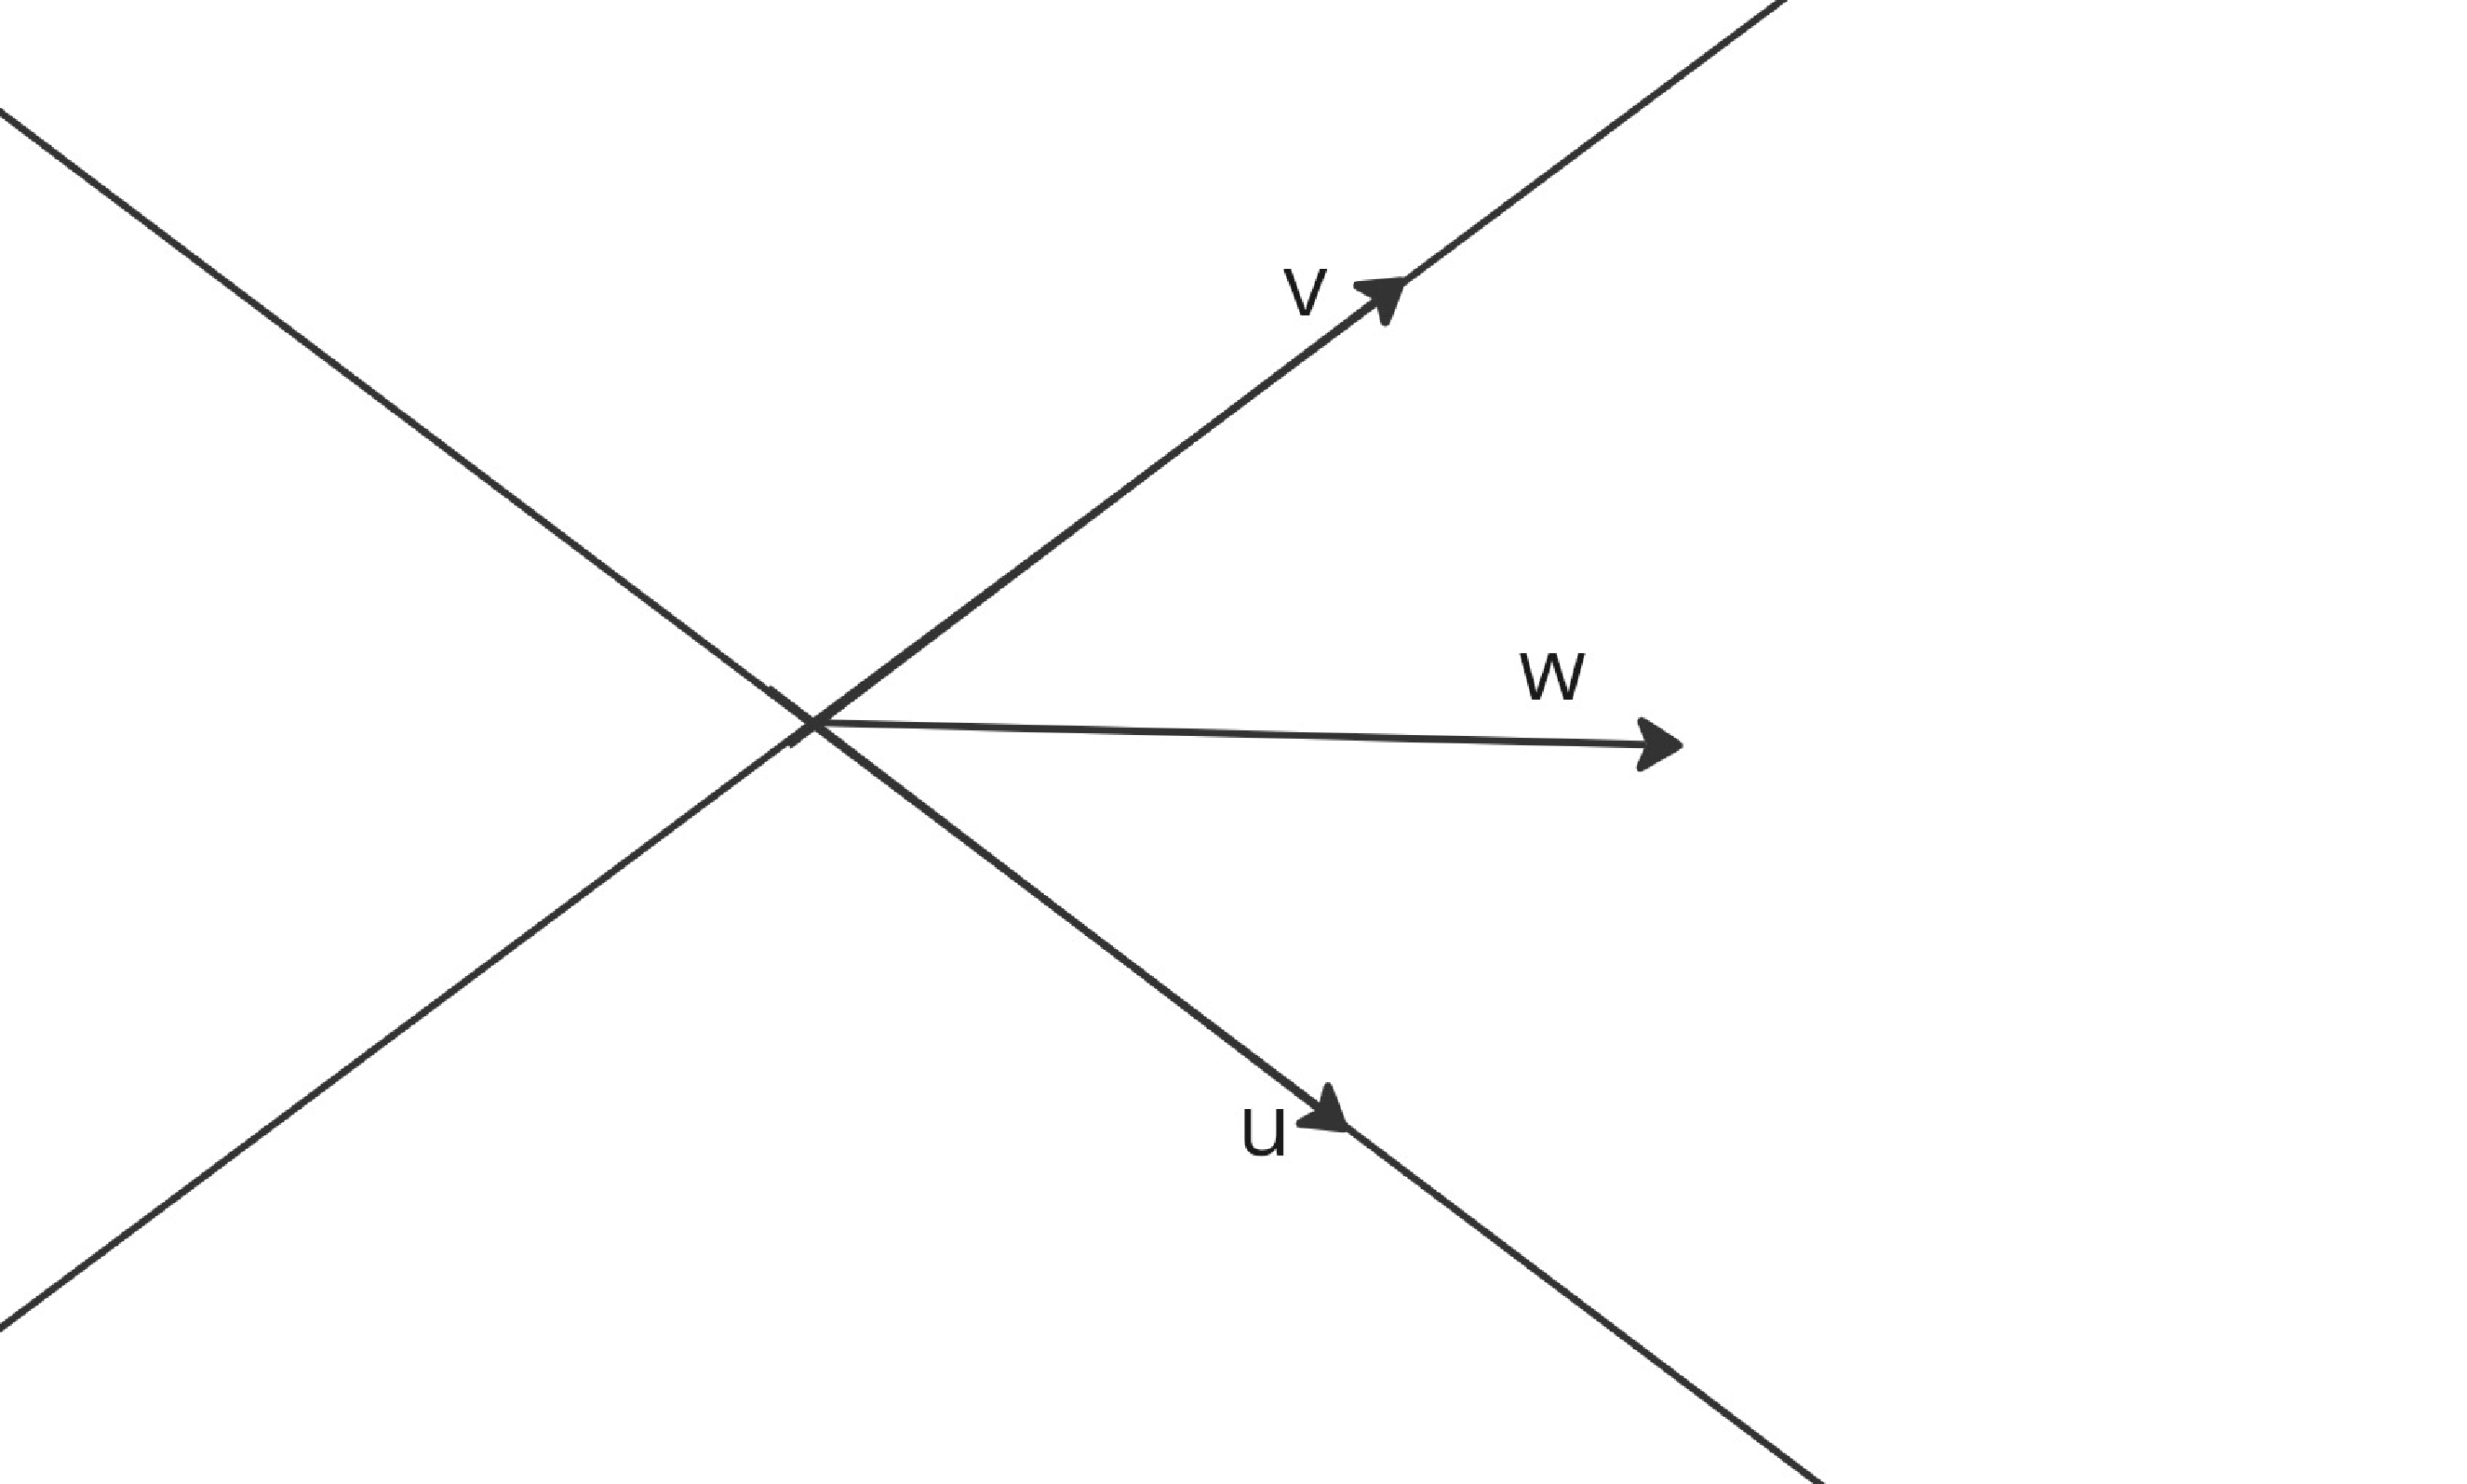
\includegraphics[scale=0.2]{algebra.pdf} 

Прямые - подпространства, v и u - вектора из объединения подпространств, их сумма w не лежит в подпространств $\Rightarrow$ их объединение не подпространство.
\end{figure}
\end{document}
